%
\documentclass{llncs} % For LaTeX2e
\usepackage{etex}
\usepackage{hyperref}
\usepackage{algorithmicx}
\usepackage[ruled,vlined]{algorithm2e}
\usepackage{pgfplots}
\usepackage{url}
\usepackage{	}
\usepackage[justification=centering]{subcaption}
\usepackage[margin=1in]{geometry}
\usepackage{amsmath,amssymb}
\usepackage{mathtools}
\usepackage{booktabs}

\usetikzlibrary{bayesnet}
\pgfplotsset{compat=newest}


\newcommand\fixme[1]{\textcolor{red}{#1}}

\newenvironment{loglisting}[1][htb]
{\renewcommand{\algorithmcfname}{Log listing}% Update algorithm name
  \begin{algorithm}[#1]%
}{\end{algorithm}}

\makeatletter
\algrenewcommand\ALG@beginalgorithmic{\ttfamily}
\makeatother

\title{
Click models evaluations\\
\small {(IR2 project)}
}

\author{
Luka Stout\\
\texttt{10616713} \\
\and
Finde Xumara \\
\texttt{10690832} \\
}

\newcommand{\fix}{\marginpar{FIX}}
\newcommand{\new}{\marginpar{NEW}}
\newcommand{\comment}[1]{\textit{\color{red}{#1}}}

\begin{document}

\nocite{*}
\maketitle

%\begin{abstract}
%\end{abstract}

\section{Introduction}
Modeling user behavior on a search engine result page is important for understanding users and supporting simulation experiments.
As result pages become more complex, click models have to evolve as well in order to capture additional aspects of user behavior in response to new forms of result presentation.
In recent years many models have been proposed that are aimed at predicting behaviour of web search users. 

In this project, we implement and evaluate different click models using multiple evaluation metrics and report on the performance of these click models.
The click models include the Click-Through Rate click model (CTR), Position-Based click model (PBM), Cascade click model (CM) \cite{Kempe2008}, User Browsing Model (UBM) \cite{Dupret2008}, Click Chain Model (CCM) \cite{Guo2009_CCM} and Task-centric Click Model (TCM) \cite{Zhang2011}.
The evaluation metrics we use to evaluate performance of these click models are loglikelihood, perplexity, click-through-rate prediction, relevance prediction, ranking performance and computation time. We will also analyze two different factors that might influence performance of the click models, query frequency and click entropy.
By doing this experiment we will know the performance of each different click model and this information can be helpful in the creation of new click models and used as a performance benchmark of new click model proposals.

%report organization
This report is organized as follows.
In Section~\ref{sec:methodology} we will describe different click models with their inference and evaluation algorithms used in our experiments.
The experiments and data source information will be covered in Section~\ref{sec:evaluation}, followed by an analysis of these experiments in Section~\ref{sec:analysis}.

\section{Click Models}
\label{sec:methodology}
In this section, we briefly describe their main characteristics and differences. We have implemented CTR, PBM, CM, CCM, and TCM ourselves, the UBM algorithm is taken from PyClick \cite{PyClick}. The general notation used in this report will be as follows:

\begin{table}[ht]
	\centering
	\begin{tabular}{l|lll|}
		\hline
		Symbol & Description \\
		\hline
		$u$	& Document $u$ \\
		$q$	& Query $q$ \\
		$ A $ & Attractiveness variable \\
		$ \alpha $ & Attractiveness parameter \\
		$ S $ & Satisfaction variable \\
		$ \sigma $ & Satisfaction parameter \\
		$ E $ & Examination variable \\
		$ \epsilon $ & Examination parameter \\
		$ R $ & Relevance variable \\
		$ r $ & Relevance parameter \\
		$ C $ & Click variable \\
		$ c $ & Actual click \\
		$ \mathcal{S} $ & All sessions \\
		$ s $ & A query session \\
		$ j $ & Position within a query session \\
		\hline
	\end{tabular}
	\caption{Notations used in the equations}
	\label{table:notations}
\end{table}

\subsection{Click-through Rate click model}
The most simple click model, Click-Through Rate (CTR), tries to predict relevance for a query-document pair. Relevance is the only parameter in this model which is the click-through rate formula. The inference is done by using maximum likelihood estimation (MLE) because there are no latent variables in this model. Therefore, the click probability of document at position $u$ will be:
\begin{align}
	P(C_{uq}=1) &= P(R_{uq}=1) \nonumber \\
	P(R_{u}=1) &= \frac{1}{|S_{uq}|} \sum_{s \in S_{uq}} c_{uq} \label{eq:ctr_rel}\\
	\text{where}&, S_{uq} = \{ s_q : u \in s_q \} \nonumber
\end{align}

\subsection{Position based model}
This model builds upon the CTR model. It adds a \texttt{position bias} where documents in a higher position are examined more often. A document can only be clicked if it was examined. The click probability of a document $u$ is as is defined in Equation~\ref{eq:PBM_click} where $P(R_{uq}=1)$ is defined as in Equation~\ref{eq:ctr_rel}. The values of $P(E_r=1)$ will be fixed. They are taken from \cite{eye_track} and are $[.68, .61, .48, .34, .28, .2, .11, .1, .08, .06]$. Inference of this model is done by using expectation-maximization (EM)
\begin{align}
	P(C_{uq}=1) &= P(E_{j_u}=1)P(R_{uq}=1) \label{eq:PBM_click}
\end{align}

where $j_u$ is the rank of document $u$.

\subsection{Cascade model}
Cascade model (CM) is another extension to the CTR model. It assumes that users abandon a search session after the first click and hence does not provide a complete picture of how multiple clicks arise in a query session and how to estimate document relevance from such data \cite{Kempe2008,Craswell2008}. This model introduces the \textit{cascade hypothesis}, a used examines a search result page (SERP) from top to bottom, deciding whether to click each result before moving to the next. This means ofcourse that to make a click, the user must have decided both to click and skip the ranks above. The relevance of a document is calculated in the same way as in Equation~\ref{eq:ctr_rel}. The click probability is defined as:
\begin{align}
	P(C_{uq}=1) &= P(E_{j_u}=1)P(R_{uq}=1) \label{eq:CM_click} \\
	P(E_{j_u}=1) &= \prod_{i=1}^{j_u-1} 1 - P(C_{i_u}=1) \nonumber
\end{align}
The inference of the parameters of CM is done using MLE-inference.

\subsection{User Browsing Model}
In \cite{Dupret2008}, Dupret and Piwowarski propose a new click model called the User Browsing Model (UBM). The main difference between UBM and other models is that UBM takes the distance into account from the current document \(u_j\) to the last clicked document \(u_{j'}\) for determining the probability that the user continues browsing:
\[P(E_{j_u} = 1 \mid C_{u_{j'}}=1, C_{u_{j'+1}}=0, \dots, C_{u_{j-1}q}=0) = \gamma_{jj'}\]

A graphical representation of the model is presented in Figure~\ref{fig:ubm_gm}.

\begin{figure}[ht!]
	\begin{center}
		\begin{tabular}{c}
			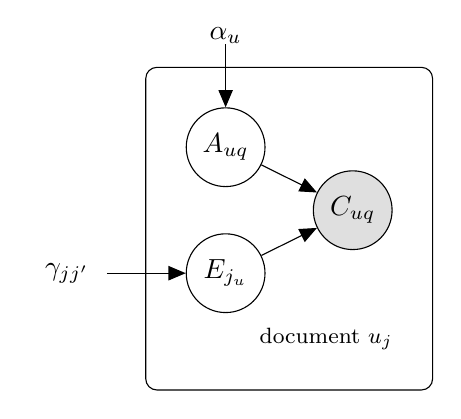
\begin{tikzpicture}
			
			% Define nodes
			\node[obs, minimum size=1cm]                      				(c) {$C_{uq}$};
			\node[latent, left=.6cm of c, yshift=.8cm, minimum size=1cm]  	(a) {$A_{uq}$};
			
			\node[latent, left=.6cm of c, yshift=-.8cm, minimum size=1cm]  	(e) {$E_{j_u}$};	
			\node[const, above=.8cm of a]  									(a_u) {$\alpha_u$};
			
			\node[const, left=1cm of e, minimum size=1cm]  	(e_p) {$\gamma_{jj'}$};	
			
			% Connect the nodes
			\edge {a,e} {c} ; %
			\edge {e_p} {e} ; %
			\edge {a_u} {a} ; %
			
			% Plates
			\plate [inner sep=.5cm, text centered] {u_j} {(a)(e)(c)} {document $u_j$};
			
			\end{tikzpicture}
		\end{tabular}
	\end{center}
	\caption{The graphical model of UBM. \fixme{PLACE THIS SIDE BY SIDE WITH CCM}}	
	\label{fig:ubm_gm}
\end{figure}

\subsection{Click Chain Model}
In \cite{Guo2009_CCM}, Fan Guo et al, proposed a bayesian based click model which was based on position bias assumption, named Click chain model (CCM). 
CCM has the following assumptions, some of which are shared with the cascade model.
\begin{enumerate}
	\item Users are homogeneous: their information needs are similar given the same query; 
	\item Decoupled examination and click events: click probability is solely determined by the examination probability and the document relevance at a given position; 
	\item Cascade hypothesis: examination is in strictly sequential order with no breaks.
\end{enumerate}

The intuition behind CCM is that the chance that a user continues after a click depends on the relevance of the previous document and that a user might abandonthe search after a while. This model can be formalized with the following conditional probabilities:
\begin{align}
	P(C_{uq}=1|E_{j_u}=0) &= 0 \nonumber\\
	P(C_{uq}=1|E_{j_u}=1, R_{uq}) &= R_{uq} \nonumber\\
	P(E_{j_u+1}=1|E_{j_u}=0) &= 0 \nonumber\\
	P(E_{j_u+1}=1|E_{j_u}=1,C_{uq}=0) &= \tau_1 \nonumber\\
	P(E_{j_u+1}=1|E_{j_u}=1,C_{uq}=1,R_{uq}) &= \tau_2(1-R_{uq})+\tau_3 R_{uq} \label{eq:ccm_simplified}
\end{align}

As $\tau_2$ and $\tau_3$ are only used in Equation~\ref{eq:ccm_simplified} and in cojunction with eachother and the relevance of the previous document we have decided to combine them into one parameter, $\tau_{click}$ and $\tau_1$ has been renamed to $\tau_{no\_click}$.

A graphical representation of the model is presented in Figure~\ref{fig:ccm_gm}.

\begin{figure}[ht!]
	\begin{center}
		\begin{tabular}{c}
			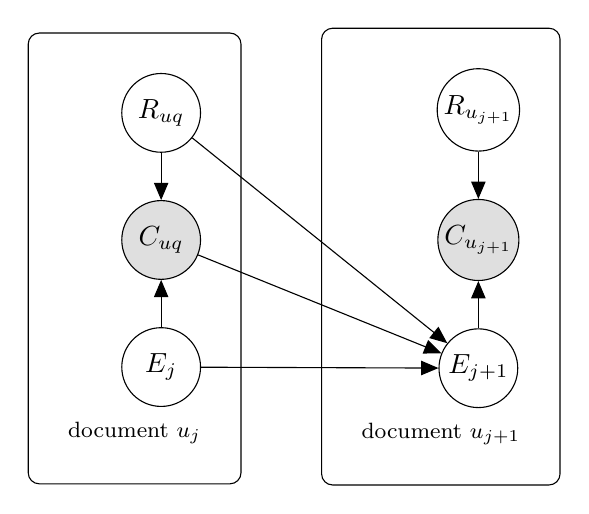
\begin{tikzpicture}
			
			% Define nodes
			\node[obs, minimum size=1cm]                      	(c) {$C_{uq}$};
			\node[latent, above=.6cm of c, minimum size=1cm]  	(a) {$R_{uq}$};			
			\node[latent, below=.6cm of c, minimum size=1cm]  	(e) {$E_j$};	
			
			\node[obs, minimum size=1cm, right=3cm of c]        (c_1) {$C_{u_{j+1}}$};
			\node[latent, above=.6cm of c_1, minimum size=1cm]  (a_1) {$R_{u_{j+1}}$};		
			\node[latent, below=.6cm of c_1, minimum size=1cm] 	(e_1) {$E_{j+1}$};	

			%\node[const, above=.8cm of a]  									(a_u) {$\alpha_u$};
			%\node[const, left=1cm of e, minimum size=1cm]  	(e_p) {$\gamma_{jj'}$};	
			
			% Connect the nodes
			\edge {a,e} {c} ; %
			\edge {a,e,c} {e_1} ; %
			%\edge {e_p} {e} ; %
			%\edge {a_u} {a} ; %
			\edge {a_1,e_1} {c_1} ; %
			
			% Plates
			\plate [inner sep=.5cm, text centered] {u_j} {(a)(e)(c)} {document $u_j$};
			\plate [inner sep=.5cm, text centered] {u_j_1} {(a_1)(e_1)(c_1)} {document $u_{j+1}$};
			
			\end{tikzpicture}
		\end{tabular}
	\end{center}
	\caption{The graphical model of CCM. \fixme{PLACE THIS SIDE BY SIDE WITH UBM}}	
	\label{fig:ccm_gm}
\end{figure}

\subsection{Task-centric Click Model}
\label{sec:methodology_tcm}
The Task-centric Click Model (TCM) was first proposed by Zhang et al. in \cite{Zhang2011}. In the paper they propose a new click model which can handle multiple clicks of multiple queries in a task by introducing two new biases. The first bias indicates that users tend to express their information needs incrementally in a task, thus perform more clicks as their needs become clearer. The other bias indicates that users tend to click fresh documents that are not included in the results of previous queries. In their paper, they named the first assumption as \texttt{query bias}, and the second assumption as \texttt{duplicate bias}. A graphical representation of the state-of-the-art of the model is presented in Figure~\ref{fig:dcm_gm} and the notations used in TCM are described in Table~\ref{table:tcm_notations}. 

\begin{table}[ht]
	\centering
	\begin{tabular}{l|lll|}
		\hline
		Symbol & Description \\
		\hline
		$M_q$			& Whether the query $q$ matches the user's intent.\\
		$N_q$ 			& Whether the the user submits another query after $q$ session.\\		
		$H_{uq}$ 		& Previous Examination of the document $u$ in query $q$.\\
		$F_{uq}$ 		& Freshness of the document $u$ in query $q$.\\
		$u'q'$ & $q'$ is the latest query session where \(u\) has appeared in previous query sessions \\
		\hline
	\end{tabular}
	\caption{Additional notations used in TCM}
	\label{table:tcm_notations}
\end{table}

This model can be formalized with the following conditional probabilities:
\begin{align}
	P(M_q=1) &= \tau_1 \\
	\label{eq:alpha_2}
	P(N_q|M_q=1) &= \tau_2 \\
	P(F_{uq}=1|M_{uq}=1) &= \tau_3 \\
	P(E_{uq}=1) &= \epsilon_j \\
	P(R_{uq}=1) &= r_u \\
	M_q = 0 &\Rightarrow N_i = 1\\
	H_{uq} = 0 &\Rightarrow F_{uq} = 1\\
	H_{uq} = 0 &\Leftrightarrow H_{u',q'} = 0, E_{u',q'} = 0\\
	C_{uq} = 1 &\Leftrightarrow M_q = 1, E_{uq} = 1, R_{uq} = 1, F_{uq} = 1
\end{align}

In our implementation, we simplified TCM model by assuming that a query matches a users intent ($M_q$) is observed from the click log data, if a user clicks in a result in a query then that query matched the users intent. thus eq.\ref{eq:alpha_2} can be removed. 
Our second assumption is that $M_q, E_{uq},R_{u}$ and $F_{uq}$ are independent. 
The detailed calculation for updating EM parameters of the simplified TCM can be found in the appendix.
The graphical model of our TCM implementation is presented in Figure~\ref{fig:tcm_gm_new}.

\begin{figure}[ht]
	\begin{subfigure}[b]{.45\textwidth}
		\centering
		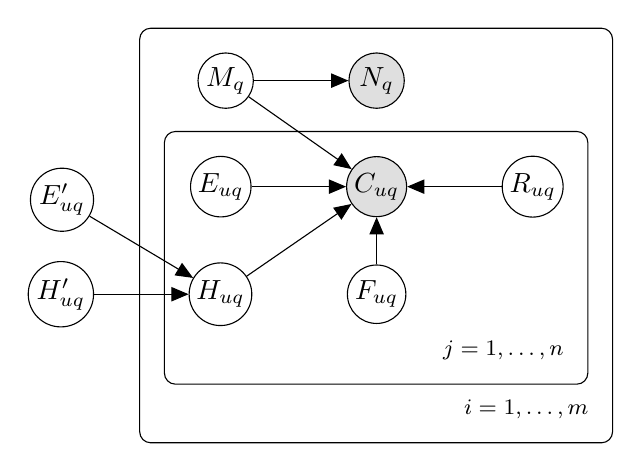
\begin{tikzpicture}
		
		% Define nodes
		\node[obs]                      (n) {$N_q$};
		\node[latent, left=1.2cm of n]  (m) {$M_q$};
		\node[obs, below=0.6cm of n]    (c) {$C_{uq}$};
		\node[latent, left=1.2cm of c]  (e) {$E_{uq}$};
		\node[latent, right=1.2cm of c] (r) {$R_{uq}$};
		\node[latent, below=0.6cm of c] (f) {$F_{uq}$};
		\node[latent, left=1.2cm of f]  (h) {$H_{uq}$};
		\node[latent, left=1.2cm of h]  (h_prime) {$H_{uq}'$};
		\node[latent, left=1.2cm of h, yshift=1.2cm]  (e_prime) {$E_{uq}'$};
		
		% Connect the nodes
		\edge {m} {n,c} ; %
		\edge {e,r,f} {c} ; %
		\edge {h} {c} ; %
		\edge {h_prime,e_prime} {h} ; %
		
		% Plates
		\plate [inner sep=.3cm] {p_n} {(e)(c)(r)(f)(h)} {$j=1,\dots,n$} ;
		\plate [inner sep=.3cm] {p_m} {(m)(n)(p_n)} {$i=1,\dots,m$} ;
		
		\end{tikzpicture}
		\caption{State-of-the-art TCM}
		\label{fig:tcm_gm}
	\end{subfigure}
	\hfill
	\begin{subfigure}[b]{.45\textwidth}
		\centering
		\begin{tikzpicture}
	
		% Define nodes
		\node[obs]					  (c) {$C_{uq}$};
		\node[obs, left=1.2cm of n, yshift=1.4cm]  (m) {$M_i$};
		\node[latent, left=1.2cm of c]  (e) {$E_{uq}$};
		\node[latent, right=1.2cm of c] (r) {$R_{uq}$};
		\node[latent, below=0.6cm of c] (f) {$F_{uq}$};
		\node[latent, left=1.2cm of f]  (h) {$H_{uq}$};
		\node[latent, left=1.2cm of h]  (h_prime) {$H_{uq}'$};
		\node[latent, left=1.2cm of h, yshift=1.2cm]  (e_prime) {$E_{uq}'$};
		
		% Connect the nodes
		\edge {m} {n,c} ; %
		\edge {e,r,f} {c} ; %
		\edge {h} {c} ; %
		\edge {h_prime,e_prime} {h} ; %
		
		% Plates
		\plate [inner sep=.3cm] {p_n} {(e)(c)(r)(f)(h)} {$j=1,\dots,n$} ;
		\plate [inner sep=.3cm] {p_m} {(m)(n)(p_n)} {$i=1,\dots,m$} ;
		
		\end{tikzpicture}
		
		\caption{Simplified TCM}
		\label{fig:tcm_gm_new}
	\end{subfigure}
	\caption{The graphical model of state-of-the-art TCM and simplified TCM.}
\end{figure}

\section{Evaluation Measures}
\label{sec:evaluation}
%Evaluation:
%	Purpose of the evaluation
%	Data used in the evaluation
%	Evaluation setup
%	Results (present as many results as necessary to illustrate the work you have done on the project - tables are a good way and required by the assignment; plots can be another good way)
To equally evaluate each click model's performance, we use evaluation metrics that have been proposed in the papers accompanying the proposals of these click models
. The evaluation metrics used in this experiment are listed below:

\subsection{Loglikelihood}
Loglikelihood is the default evaluation metric in machine learning. It says something about the likelihood of the data give the model. In Equation~\ref{eq:loglikelihood} the calculation of the loglikelihood of a click model and a set of sessions can be seen, where $\mathcal{L}\mathcal{L}(S|\mathbf{M})$ is the loglikelihood of the sessions given the models parameters, $S$ the set of sessions, $\mathbf{M}$ the model and its parameters, $r$ is the rank of a particular document in a session and $c_r^{(s)}$ a indicator function that is $1$ when the document at rank $r$ in session $s$ was clicked and $0$ otherwise.
\begin{align}
	\mathcal{L}\mathcal{L}(S|\mathbf{M}) = \frac{1}{|S|}\sum_{s \in S} \frac{1}{|s|} \sum_{r = 1}^{|s|} \log P(C_r=c_r^{(s)}|\mathbf{M}, C_{r-1}, C_{r-2}\dots C_1)
	\label{eq:loglikelihood}
\end{align}

\subsection{Perplexity}
Click perplexity is a widely used metric for evaluating click model accuracy. It measures how surprised a model is to see $c_r^{(s)}$ under the current parameters. Perplexity is calculated for every rank individually, as to see whether some models perform better on documents higher on the SERP page then documents ranked lower on the SERP. It is used as a evaluation metric in \cite{Zhang2011} and \cite{Dupret2008}. The calculation of perplexity can be seen in Equation~\ref{eq:perplexity}.
\begin{align}
	Perplexity_r &= 2^{-\frac{1}{|S|} \sum_{s \in S}(c_r^{(s)} \log_2 p_r + (1-c_r^{(s)} ) \log_2 (1-p_r))} \label{eq:perplexity} \\
	p_r &= P(C_r = 1 | \mathbf{M}) \nonumber
\end{align}
The perplexity of a model is defined as the average of perplexities over all positions. Thus, a smaller perplexity value indicates a better consistency between the click model and the actual click data.

\subsection{Click-Trough-Rate Prediction (CTR)}
\label{sec:ctr}
The purpose of click-through rates is to measure the ratio of clicks to impressions of an document.
Generally the higher the CTR the higher chance of that document being clicked.
The click-through rate of a document $d$ is defined as:
\begin{align}
	CTR_d = \frac{1}{|S_d|} \sum_{s_d} c_{r_d}^{(s_d)}
\end{align}
where $S_d$ is the set of sessions where document $d$ appears.
A way to use this as an evaluation measure is proposed in \cite[p. 4]{Chapelle2009}. In the same way we calculate the CTR prediction using the following protocol:
\begin{enumerate}
	\item Retrieve all sessions related to a given query.
	\item Consider an url that appears both in position 1 and some other positions.
	\item Hold out as test sessions all the sessions in which that url appeared in position 1.
	\item Train the model on the remaining sessions and predict the relevance.
	\item Compute the test CTR in position 1 on the held-out sessions.
	\item Compute an error between these two quantities.
	\item Average the error on all such urls and queries, weighted by the number of test sessions.
\end{enumerate}

The error measure we use is the Root-Mean-Square-Error (RMSE).

\subsection{Relevance Prediction}
Relevance prediction was used to evaluate performance of the DBN model \cite[p. 6]{Chapelle2009}.
The accuracy of CTR prediction may not directly translate to relevance, especially when we were to evaluate the whole task instead of a single query.
In this case, the CTR of a particular document is highly dependent on the user-model assumptions.
For example if a user tends to ignore a document that isn't fresh, the CTR will be low even if the document is relevant.
To measure relevance prediction we use a hand annotated set of relevances. This set contains for a group of query-document pairs a relevance. For these pairs we use the models to predict the relevance. We then use the Area Under the Curve (AUC) between the annotated relevances and the predicted relevances as an evaluation measure. We also calculate the pearson-correlation between the two.

\subsection{Predicted Relevance as a Ranking Feature}
In this set of experiments we use the predicted relevance directly to rank urls, we use the model as a ranker. To evaluate the performance of a ranker we use the Normalized Discounted Cumulative Gain (NDCG) \cite{NDCG}, for which we use a cutoff at five (NDCG@5). To calculate the NDCG@5 we only consider the documents for which we have annotated relevances. All these queries are then averaged to calculate the ranking performance of the click model. The algorithm can be seen below:

\begin{enumerate}
	\item Retrieve all session that appear more than 10 times.
	\item Filter out the sessions that don't appear in the editorial judgements.
	\item Train the model on the sessions and predict relevance for the sessions.
	\item Sort the urls w.r.t the predicted relevance given by the model.
	\item Compute the NDCG@5.
	\item Average over all sessions.
\end{enumerate}

\subsection{Computation Time}
Historically in machine learning a big problem in creating accurate models was the amount of data that was available. However this is no longer the case, we are mostly restricted by the time that it takes to learn a model from the large amount of data that we currently have. This make the ability to efficiently compute parameters an important feature of a succesful model. Therefore we also decided to look at the computation time it takes to train the click models.

\section{Analysis}
\label{sec:analysis}
%Analysis
After running the experiments we were able to evaluate the different algorithms based on the ...

\section{Conclusion}
\label{sec:conclusion}
%Conclusions
In this paper we showed that ...

In our implementation, we did not ...


\bibliography{references}{}
\bibliographystyle{plain}

\newpage
\appendix
\section{Appendix}
\label{app:tcm_eq}
We give here some details about the inference in our TCM implementation outlined in section \ref{sec:methodology_tcm}.

\subsection{Click probability}
For $P(F_{i,j}=1)$ we introduce a variable $f_{i,j}$, which will be derived later. \\
By assumption that $M_i, E_{i,j},R_{i,j}$and$F_{i,j}$ are independent, click probability can be formularize as:
\begin{align}
P(C_{i,j} = 1)
&= P(M_i=1) * P(E_{i,j}=1) * P(R_{i,j}=1) * P(F_{i,j} = 1) \\
&= \alpha_1 * \beta_j * r_{i,j} * f_{i,j}
\label{eq:proba_click}
\end{align}

\subsection{Probability of the query match user intention}
Because we remove equation that depends on $\alpha_2$, we can now set $\alpha_1$ as MLE.
\begin{align*}
P(M_i = 1) 
&= \alpha_1 \\
\end{align*}

\subsection{Probability of user submit next query}
User submit next query if the query does not match user intention ($\alpha_1$) or user want to search more.
\begin{align*}
P(N_i=1) 
&= \frac{1}{|S|} \sum_{i\in S} \mathcal{I}(N_i=1) \\
&= \frac{q_i}{|S|} \\
&= n_i
\end{align*}

$q_i$ is the number of submitted-queries where user submit another query after $i$-th query session.

\begin{align*}
P(N_i=1|M_i=1) 
&= \alpha_2 \\
&= \frac{P(N_i=1) - P(N_i=1|M_i=0)P(M_i=0)}{P(M_i=1)} \\
&= \frac{n_i + \alpha_1 - 1}{\alpha_1}
\end{align*}

\subsection{Relevance probability}
\begin{align*}
P(R_{i,j} = 1)
&= r_{i,j} \\
&= \frac{\sum_{q_{i,j} \in S_{i,j}} P(R_{i,j}=1 | C)}{|S_{i,j}|}
\end{align*}

Where $S_{i,j}$ are all sessions (queries) containing the document corresponding with the query $i$ at rank $j$ - document
$P(R_{i,j}=1 | C)$ will be derive on eq.\ref{eq:proba_relevant_given_click}

\begin{align}
P(R_{i,j}=1 | C)
&= \mathcal{I}(C_{i,j} = 1) P(R_{i,j}|C_{i,j}=1) + \mathcal{I}(C_{i,j} = 0) P(R_{i,j}|C_{i,j}=0) \\
&= c_{i,j} + (1-c_{i,j}) \frac {P(C_{i,j}=0|R_{i,j}=1) P(R_{i,j} = 1)} {P(C_{i,j} = 0)} \\
&= c_{i,j} + (1-c_{i,j}) \frac {P(C_{i,j}=0|R_{i,j}=1) r_{i,j}} { 1 - P(C_{i,j} = 1)}
\label{eq:proba_relevant_given_click}
\end{align}
Where $c_{i,j} = 1$ if (i,j) was clicked in the current session.
$P(C_{i,j}=0|R_{i,j}=1)$ is the chance of no click given that it is relevant. 

\begin{align*}
P(C_{i,j}=0|R_{i,j}=1) 
&= P(C_{i,j }=0|R_{i,j}=1, M_i = 1) P(M_i=1) + P(C_{i,j }=0|R_{i,j}=1, M_i = 0)P(M_i=0) \\
&= \alpha_1 P(C_{i,j }=0|R_{i,j}=1, M_i = 1, E_{i,j}=1) P(E_{i,j}=1)\\     &+ \alpha_1 P(C_{i,j }=0|R_{i,j}=1, M_i = 1, E_{i,j}=0) P(E_{i,j}=0)\\
&+ (1-\alpha_1) P(C_{i,j }=0|R_{i,j}=1 , M_i = 0, E_{i,j}=1) P(E_{i,j}=1)\\
&+ (1-\alpha_1) P(C_{i,j }=0|R_{i,j}=1 , M_i = 0, E_{i,j}=0) P(E_{i,j}=0) \\
\\
&= \alpha_1 \beta_j P(C_{i,j }=0|R_{i,j}=1, M_i = 1, E_{i,j}=1, F_{i,j}=1) P(F_{i,j}=1)\\
&+ \alpha_1 \beta_j P(C_{i,j }=0|R_{i,j}=1, M_i = 1, E_{i,j}=1, F_{i,j}=0) P(F_{i,j}=0)\\
&+ \alpha_1 (1-\beta_j) P(C_{i,j }=0|R_{i,j}=1 , M_i = 1, E_{i,j}=0, F_{i,j}=1) P(F_{i,j}=1)\\
&+ \alpha_1 (1-\beta_j) P(C_{i,j }=0|R_{i,j}=1 , M_i = 1, E_{i,j}=0, F_{i,j}=0) P(F_{i,j}=0)\\
&+ (1-\alpha_1) \beta_j P(C_{i,j }=0|R_{i,j}=1, M_i = 0, E_{i,j}=1, F_{i,j}=1) P(F_{i,j}=1)\\
&+ (1-\alpha_1) \beta_j P(C_{i,j }=0|R_{i,j}=1, M_i = 0, E_{i,j}=1, F_{i,j}=0) P(F_{i,j}=0)\\
&+ (1-\alpha_1) (1-\beta_j) P(C_{i,j }=0|R_{i,j}=1 , M_i = 0, E_{i,j}=0, F_{i,j}=1) P(F_{i,j}=1)\\
&+ (1-\alpha_1) (1-\beta_j) P(C_{i,j }=0|R_{i,j}=1 , M_i = 0, E_{i,j}=0, F_{i,j}=0) P(F_{i,j}=0)\\
\end{align*}
We note that $P(C_{i,j }=0|R_{i,j}=1, M_i = 1, E_{i,j}=1, F_{i,j}=1) = 0$. Otherwise it is $1$. From eq. 24 from TCM paper. Together with inserting our parameters this gives us the following:

\begin{align}
P(C_{i,j}=0|R_{i,j}=1) &= 
\alpha_1 \beta_j f_{i,j} +
\alpha_1 \beta_j (1-f_{i,j}) + 
\alpha_1 (1-\beta_j) f_{i,j} +
\alpha_1 (1-\beta_j) (1-f_{i,j}) \\
&+ (1-\alpha_1) \beta_j f_{i,j} +
(1-\alpha_1) \beta_j (1-f_{i,j}) +
(1-\alpha_1) (1-\beta_j) (f_{i,j} \\
&+(1-\alpha_1) (1-\beta_j) (1-f_{i,j})
\end{align}

expanding this we are only left with
\begin{align}
P(C_{i,j}=0|R_{i,j}=1) = 1 - (\alpha_1 \beta_j f_{i,j})
\label{eq:chance_no_click_given_relevant}
\end{align}
Which seems intuitive as we assumed that all $M_i, R_{i,j}, E_{i,j}$ and $F_{i,j}$ are independent to get $P(C_{i,j} = 1)$ . With this information we can calculate 
\begin{align}
P(R_{i,j}=1 | C) &= c_{i,j} + (1-c_{i,j}) \frac { (1 - (\alpha_1 \beta_j f_{i,j}))  r_{i,j}} { 1 - \alpha_1 \beta_j f_{i,j} r_{i,j} } \\
&= c_{i,j} + (1-c_{i,j}) \frac{r_{i,j} - \alpha_1 \beta_j f_{i,j} r_{i,j} }{ 1 - \alpha_1 \beta_j f_{i,j} r_{i,j}}
\end{align}

\subsection{Examination probability}
\begin{align}
P(E_{i,j} = 1) 
&= \beta_j \\
&= \frac{1}{|S|} \sum_{i \in S} P(E_{i,j}=1 | C)
\end{align}
Where $S$ is all sessions and $i$ is a query within that session.
$P(E_{i,j}=1 | C)$ will be derive on eq.\ref{eq:proba_examined_given_click}

\begin{align}
\label{eq:proba_examined_given_click}
P(E_{i,j}=1 | C)
&= \mathcal{I}(C_{i,j} = 1) P(E_{i,j}|C_{i,j}=1) + \mathcal{I}(C_{i,j} = 0) P(E_{i,j}|C_{i,j}=0) \\
&= c_{i,j} + (1-c_{i,j}) \frac {P(C_{i,j}=0|E_{i,j}=1) P(E_{i,j} = 1)} {P(C_{i,j} = 0)} \\
&= c_{i,j} + (1-c_{i,j}) \frac {P(C_{i,j}=0|E_{i,j}=1) \beta_j} { 1 - P(C_{i,j} = 1)}
\end{align}
Where $c_{i,j}$ indicates whether document $i,j$ was clicked.
Analog to eq \ref{eq:chance_no_click_given_relevant} we can show that
\begin{align}
P(C_{i,j}=0|E_{i,j}=1) = 1 - (\alpha_1 f_{i,j} r_{i,j})
\end{align}

This gives us 
\begin{align}
P(E_{i,j}=1 | C) 
&= c_{i,j} + (1-c_{i,j}) \frac {( 1 - (\alpha_1 f_{i,j} r_{i,j}) )\beta_j} { 1 - \alpha_1 \beta_j f_{i,j} r_{i,j}} \\
& = c_{i,j} + (1-c_{i,j}) \frac {\beta_j - \alpha_1 \beta_j f_{i,j} r_{i,j}} { 1 - \alpha_1 \beta_j f_{i,j} r_{i,j}}
\end{align}

\subsection{Freshness probability}
\begin{align}
P(F_{i,j} = 1 | H_{i,j} = 1) &= \alpha_3 \\
\alpha_3 &= \frac{1}{|S_{i,j}|} \sum_{q \in S} \sum_{(i,j) \in q} P(F{i,j}=1 | H_{i,j}=1, C)
\label{eq:freshness}
\end{align}

Where (i,j) is a query, rank pair identifying a certain document.
$P(F_{i,j}=1 | C)$ will be derive on eq.\ref{eq:proba_freshness_given_click} \\
$P(F_{i,j}=1)$ will be derive on eq.\ref{eq:proba_freshness}

\begin{align}
\label{eq:proba_freshness_given_click}
P(F_{i,j}=1 | H_{i,j}=1, C)
&= \mathcal{I}(C_{i,j} = 1) P(F_{i,j}=1|H_{i,j}=1,C_{i,j}=1) \\
&+ \mathcal{I}(C_{i,j} = 0) P(F_{i,j}=1|H_{i,j}=1,C_{i,j}=0) \\
&= c_{i,j} + (1-c_{i,j}) \frac {P(C_{i,j}=0|F_{i,j}=1,H_{i,j}=1) P(F_{i,j} = 1 | H_{i,j}=1)} {P(C_{i,j} = 0 | H_{i,j} = 1)}
\end{align}

Analog to eq \ref{eq:chance_no_click_given_relevant} we can show that
\begin{align}
P(C_{i,j}=0|F_{i,j}=1, H_{i,j}=1) &= 1 - (\alpha_1 \beta_j r_{i,j})
\label{eq:no_click_freshness}
\end{align}
We can also show
\begin{align}
P(C_{i,j}=0|H_{i,j}=1) 
&= 1 - P(C_{i,j}=1|H_{i,j}=1) \\
&= 1-(\alpha_1 \alpha_3 \beta_j r_{i,j})
\end{align}
The only difference between this and eq.  \ref{eq:proba_click} is that it is given that $H_{i,j}=1$ and because $H_{i,j} = 1$ only has an influence on $P(F_{i,j}=1)$, namely that $P(F_{i,j}=1 | H_{i,j} = 1) = 1$, we can substitute $f_{i,j}$ with $\alpha3$ in eq. \ref{eq:proba_click}\\
\\
Now we only need to calculate $f_{i,j} = P(F_{i,j}) = 1$
\begin{align}
\label{eq:proba_freshness}
P(F_{i,j} = 1)
&= \mathcal{I}(H_{i,j}=1) P(F_{i,j}=1|H_{i,j}=1) + \mathcal{I}(H_{i,j}=0) P(F_{i,j}=1|H_{i,j}=0) \\
&= \mathcal{I}(H_{i,j}=1) \alpha_3 + \mathcal{I}(H_{i,j}=0)
\end{align}
Where $\mathcal{I}(H_{i,j}=1)$ is a binary indicator function from the data specifying whether document $(i,j)$ was shown before in the current ($q$ from eq. \ref{eq:freshness}) session.\\

We could replace this indicator function with the probability that the document was examined the last time it was shown. This probability, called $H_{i,j}$ would depend on the probability that it was examined and $H_{i',j'}$ where $i',j'$ is the last time this document was shown in the current session. It would look like this

\begin{align}
P(H_{i,j} = 1) 
&= P(E_{i',j'} = 1) P(H_{i',j'} = 1)
\end{align}

then eq. \ref{eq:proba_freshness} becomes: 
\begin{align}
P(F_{i,j} = 1) 
&= P(H_{i,j}=1) \alpha_3 + P(H_{i,j}=0) \\
&= P(H_{i,j}=1) \alpha_3 + (1 - P(H_{i,j}=1)) \\
&= \alpha_3 P(E_{i',j'} = 1) P(H_{i',j'} = 1) + (1 -  P(E_{i',j'} = 1) P(H_{i',j'} = 1))
\end{align}
Note that this discards the information that if $(i',j')$ was clicked it surely was examined. 

With eq \ref{eq:no_click_freshness} we can calculate $P(F_{i,j}=1 | C)$
\begin{align}
P(F_{i,j}=1 | H=1, C) 
&= c_{i,j} + (1-c_{i,j}) \frac {(1 - (\alpha_1 \beta_j r_{i,j})) \alpha_3} { 1 - \alpha_1 \alpha_3 \beta_j r_{i,j}} \\
&= c_{i,j} + (1-c_{i,j}) \frac {\alpha_3 - \alpha_1 \alpha_3 \beta_j r_{i,j}}{ 1 - \alpha_1 \alpha_3 \beta_j r_{i,j}}
\end{align}


\end{document}
